\documentclass{article}

\usepackage{geometry}
\geometry{a4paper, scale=0.8}

\usepackage{graphicx}
\usepackage{float}

\usepackage{ctex}

\title{ISOA Progress Report 2}
\author{Group "200"\\YiDai 2017013562\\ZhaohengLi 2017050025}

\begin{document}
\maketitle
\section{项目介绍}
我们以疫情部分的舆论方面为核心,提取舆论主题,结合时间线展示群众的关注点变化,对访问者提供舆论谣言判断服务。同时我们也注意到,信息服务平台如果缺失一方面的关键信息很容易丧失吸引力,我们还会实现政府的相关措施发布、并实现确诊数据展示。

主要实现目标如下:
\begin{itemize}
	\item{\textbf{疫情展示}} 主要包括疫情确诊地图、详细数字和相关新闻或政策的时间线。
	\item{\textbf{舆情关注展示}} 对舆情进行主题提取,结合时间线展示群众的关注点变化
	\item{\textbf{虚假新闻/谣言判断及搜索}} 用户输入文本,对文本进行分析,为用户提供相关已证实谣言或者相关新闻,并给出用户输入文本为谣言的概率。
\end{itemize}

项目计划:
\begin{figure}[H]
\centering
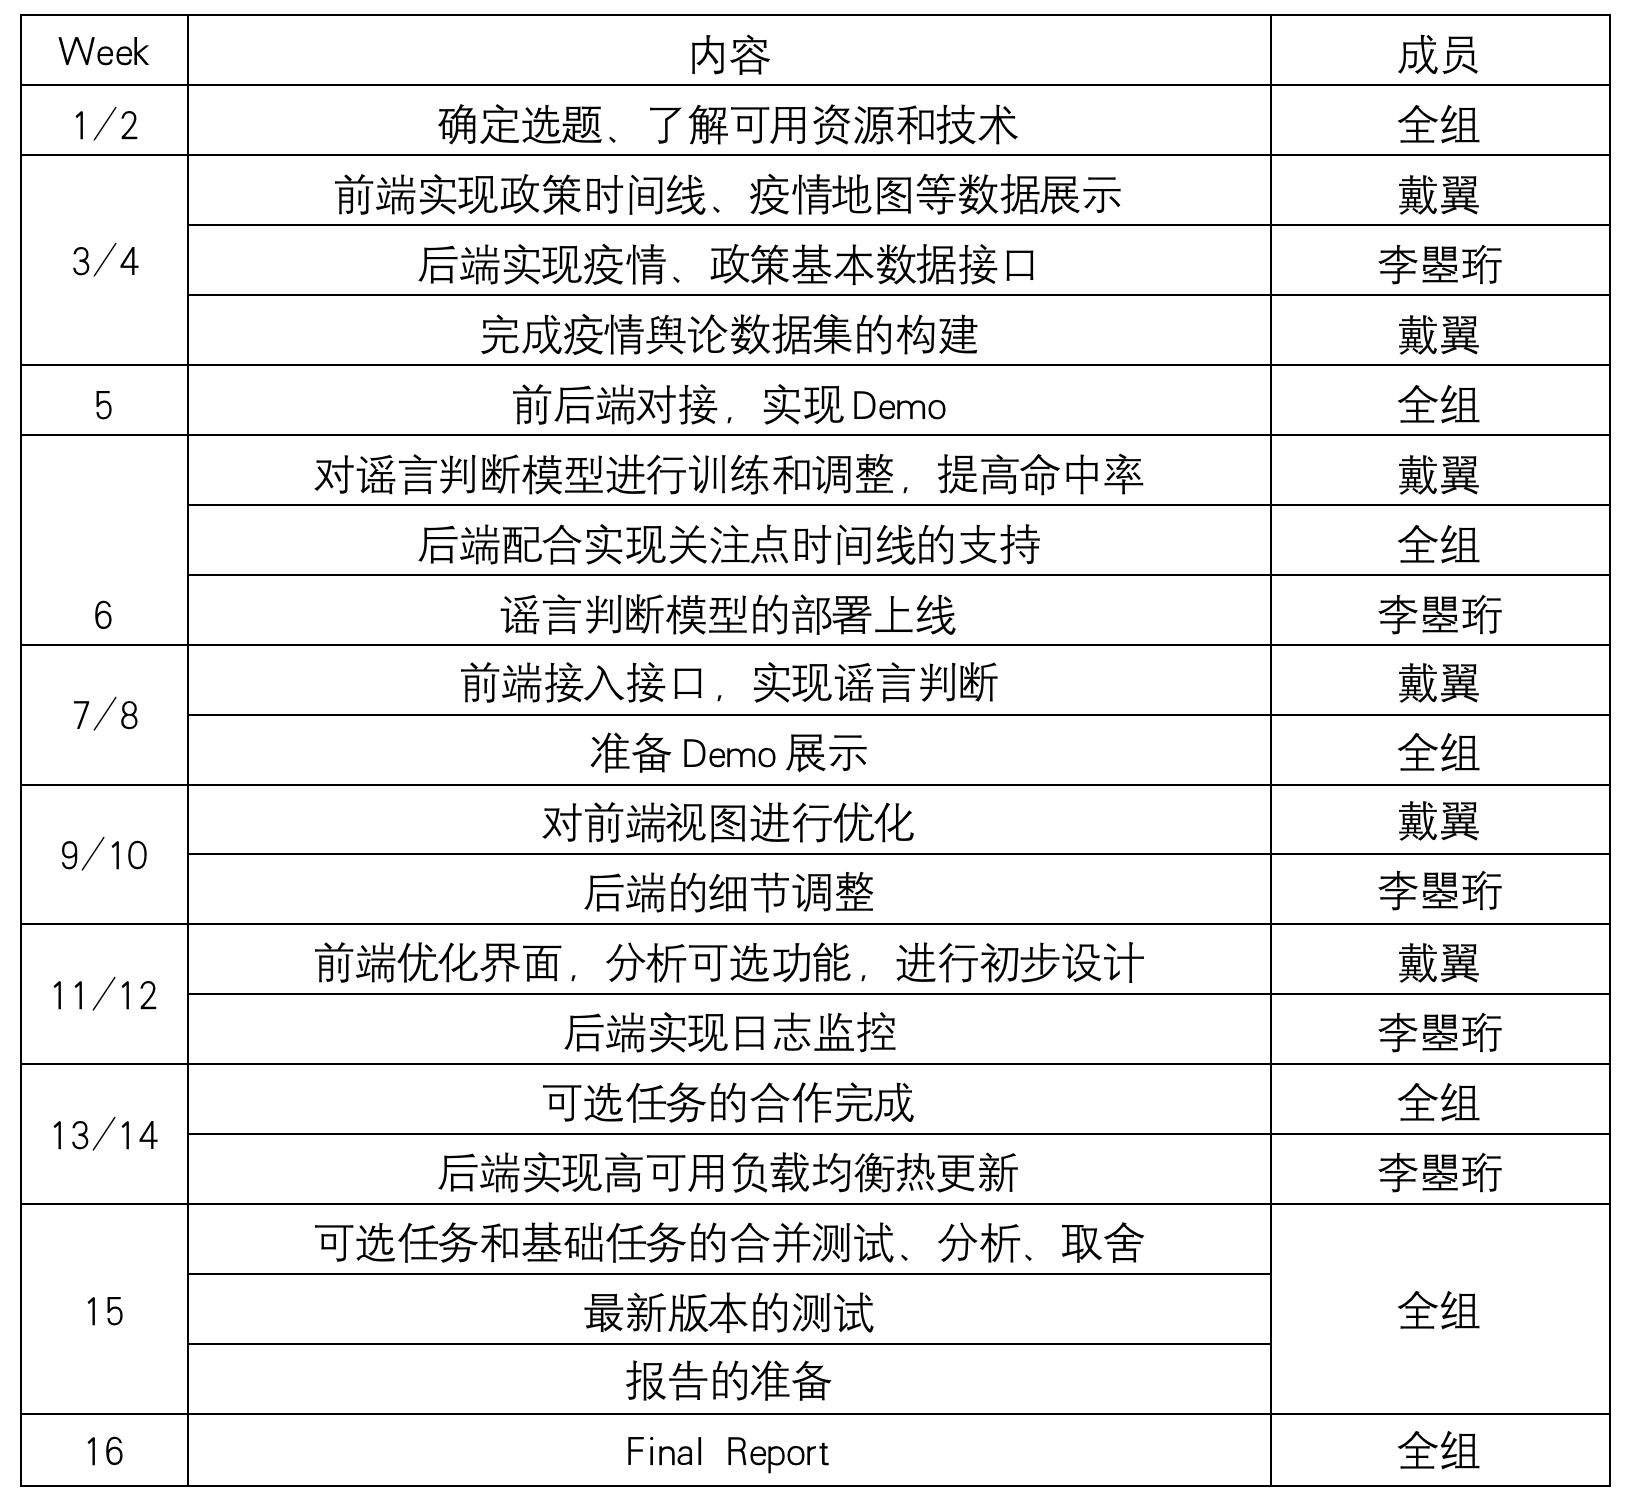
\includegraphics[width=0.6\textwidth]{pic1.png}
\end{figure}


\section{针对中期反馈作出的改进}

\subsection{舆论数据的丰富}

在前一阶段中,我们发现我们的舆论数据内容较为单一,因此我们从微博上爬取相关的新闻、用户的评论等信息来丰富我们的数据库,并进一步完善了原有的筛选算法。

我们从新浪微博中爬取了人民日报账号下关于新冠病毒的相关新闻约4000条文本,加入了我们的舆论数据库中,使舆论热点部分分析的语料库更加丰富,同时对热点词的抽取算法做了一些改进。


\subsection{前端用户体验的改善}

在中期报告中,用户提出了一系列的体验感受和建议,其中最重要的就是信息加载时的空白屏现象。一般前端开发者有“可能触发用户等待行为的操作”的说法,我们将这类切换都加上了过渡动画,并进一步缩短了加载时间。

之前还有用户线下反馈了点击全国地图省区无法直接跳转到目标省份地图的问题,我们也进行了修复。



\begin{figure}[H]
\centering
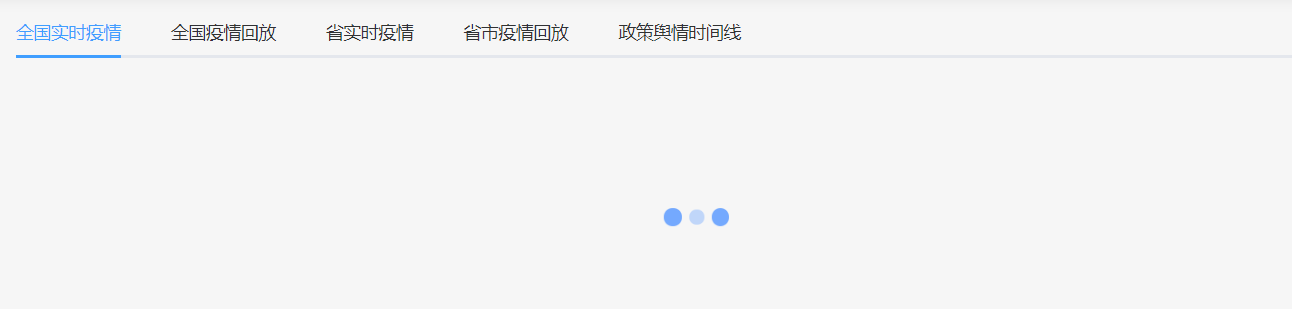
\includegraphics[width=0.8\textwidth]{pic5.png}
\end{figure}

\subsection{前端视图和互动优化}

我们在中期报告中发现JustDropIt组采用的词云展示性更好,我们在之前的词云上加了随机颜色处理,并且加上了云状外框。

我们还发现目前的界面互动性不够充分,目前采用弹幕+文本框的方式,也是一个辅助谣言判断的新功能:用户可以看到使用者群体的查询信息、上传和阅览相关的信息更新,实现一个扁平的“社区”。该功能我们正在向同学调研体验。

\begin{figure}[H]
\centering

\includegraphics[width=0.8\textwidth]{pic6.png}
\end{figure}

\begin{figure}[H]
\centering

\includegraphics[width=0.8\textwidth]{pic7.png}
\end{figure}



\section{项目的日志记录}
\subsection{后端的日志}
\subsubsection{站点访问日志}
由于整个后端是使用Flask包装而成的,因此对于后端站点访问的日志是十分重要的。我们在日志中记录了每一次访问的来源、时间、接口和结果等信息,下图为部分记录。

\begin{figure}[H]
\centering
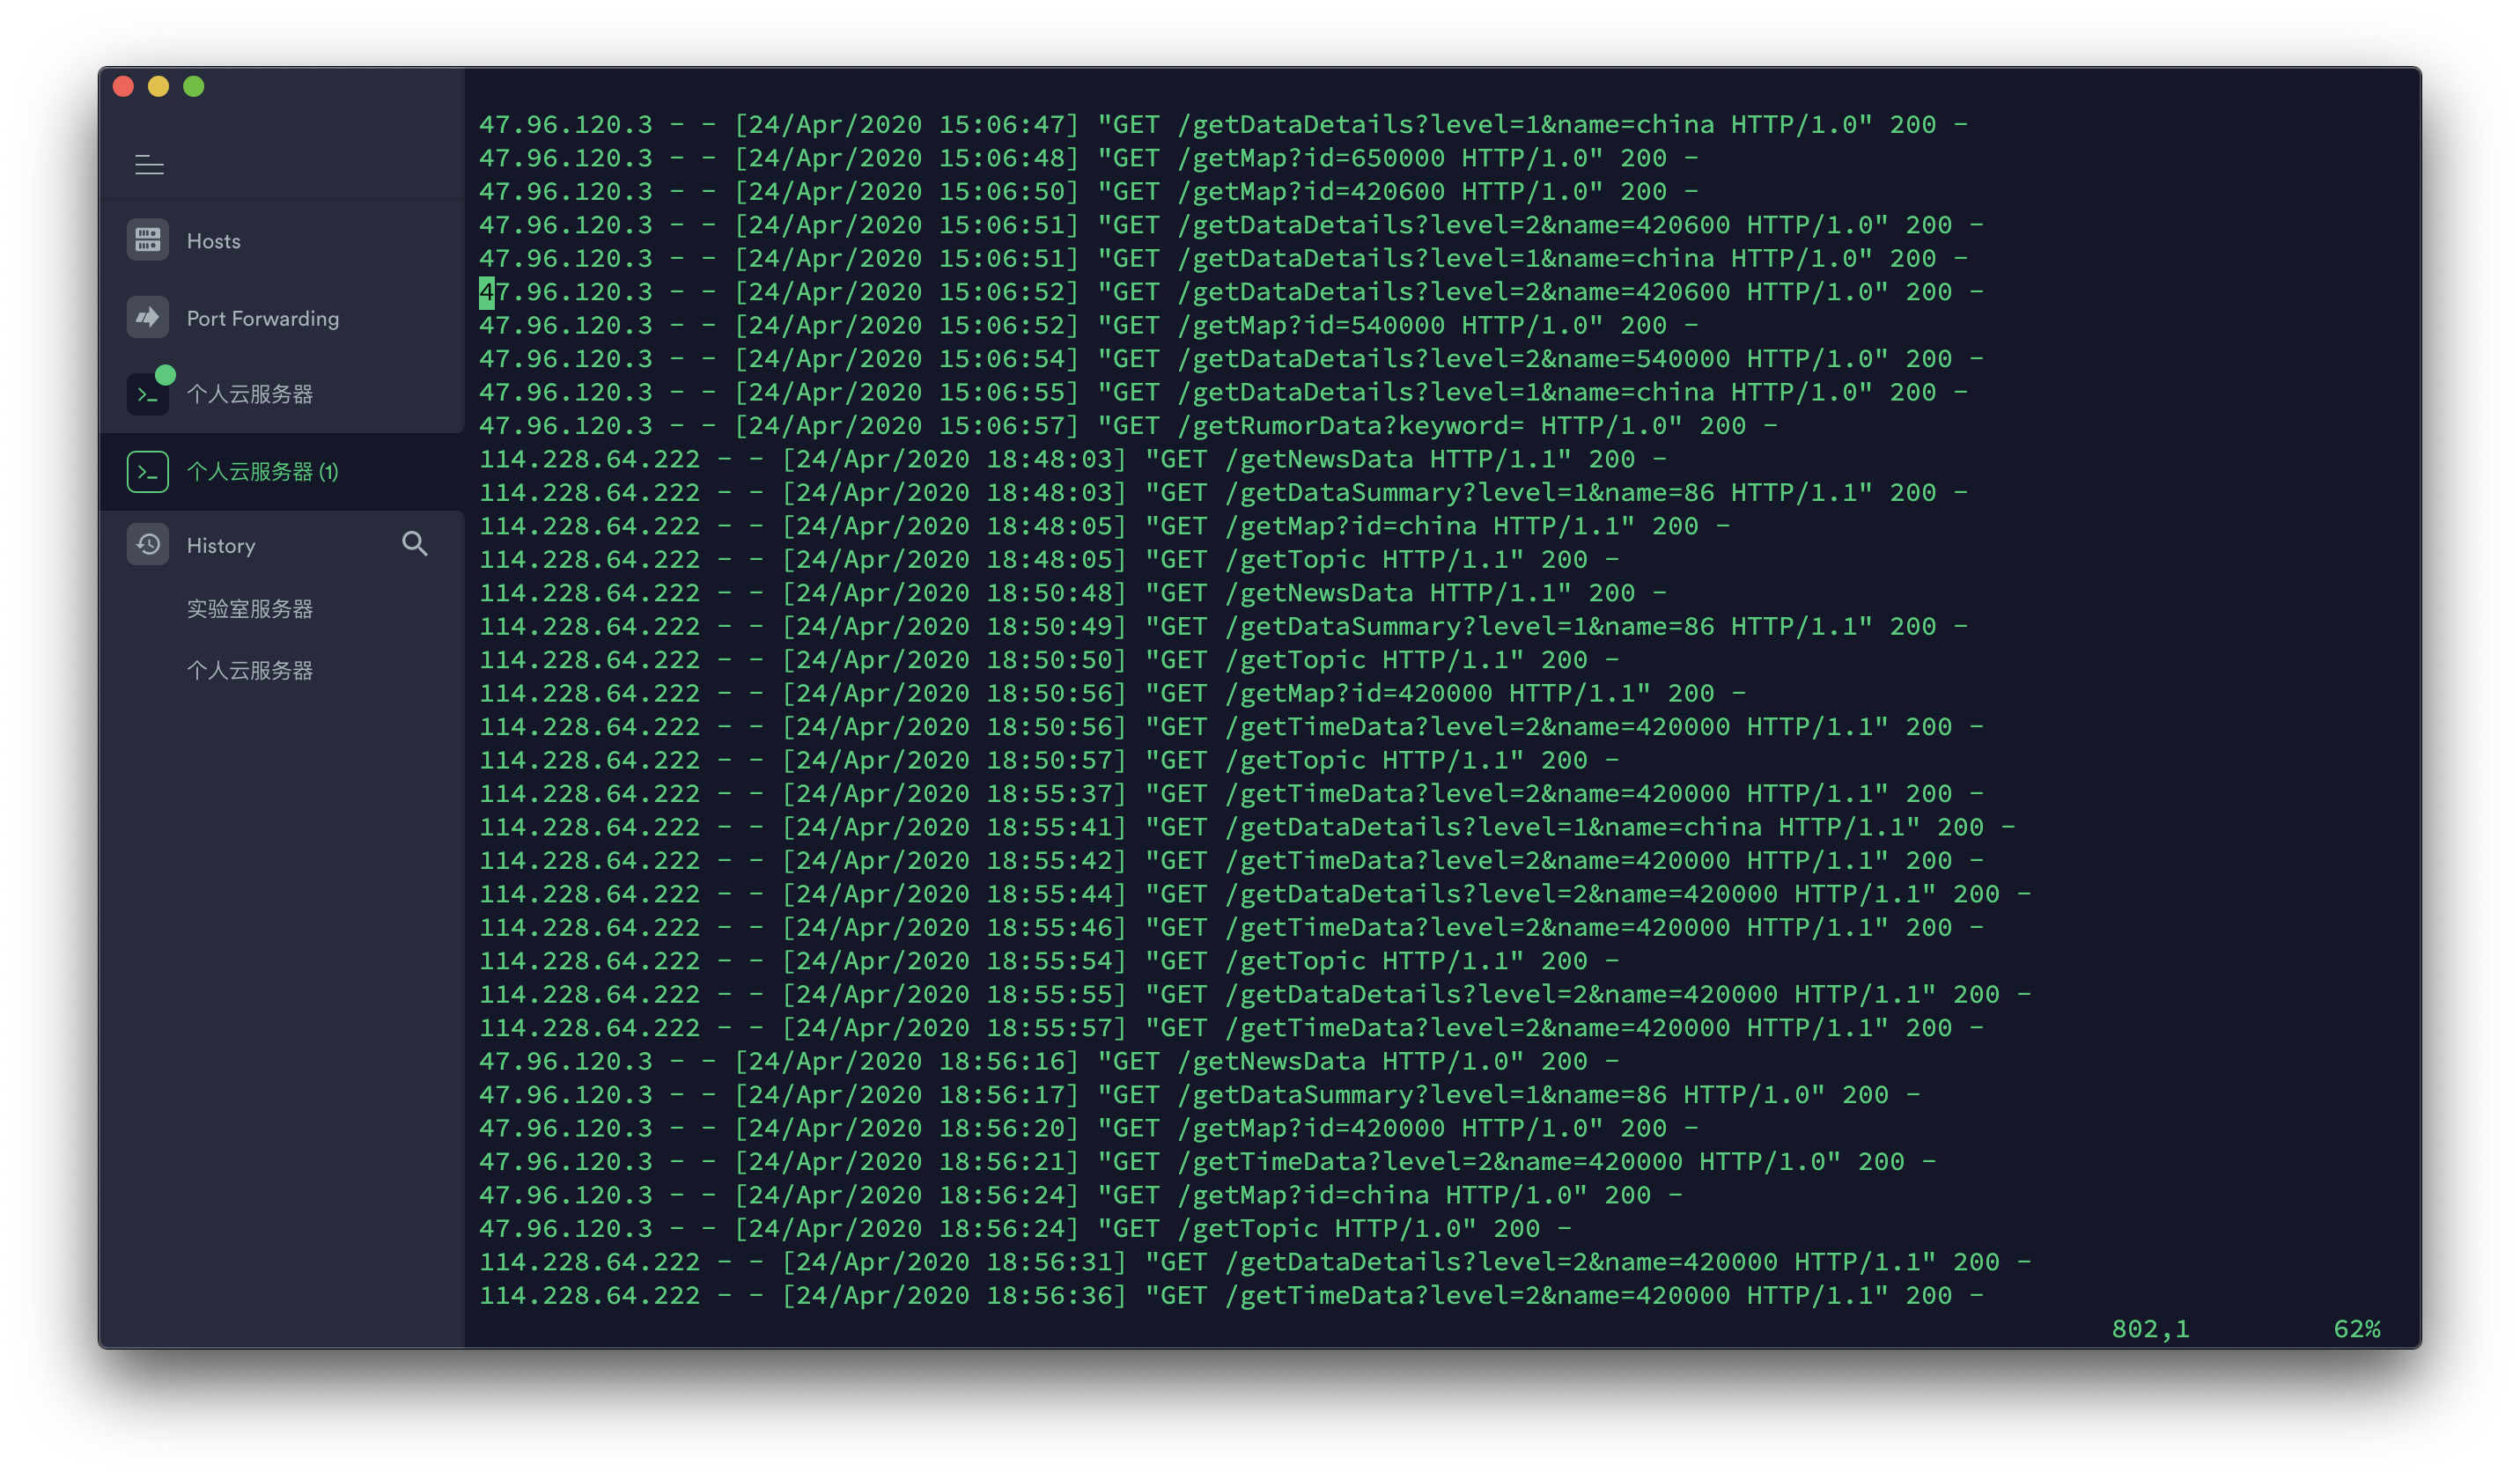
\includegraphics[width=0.8\textwidth]{pic2.png}
\end{figure}

通过站点访问日志我们可以清楚地了解到后端的整体运行情况,并且可以从日志中发现我们项目中的一些问题。例如之前站点访问日志出现了如下条目:

\begin{figure}[H]
\centering
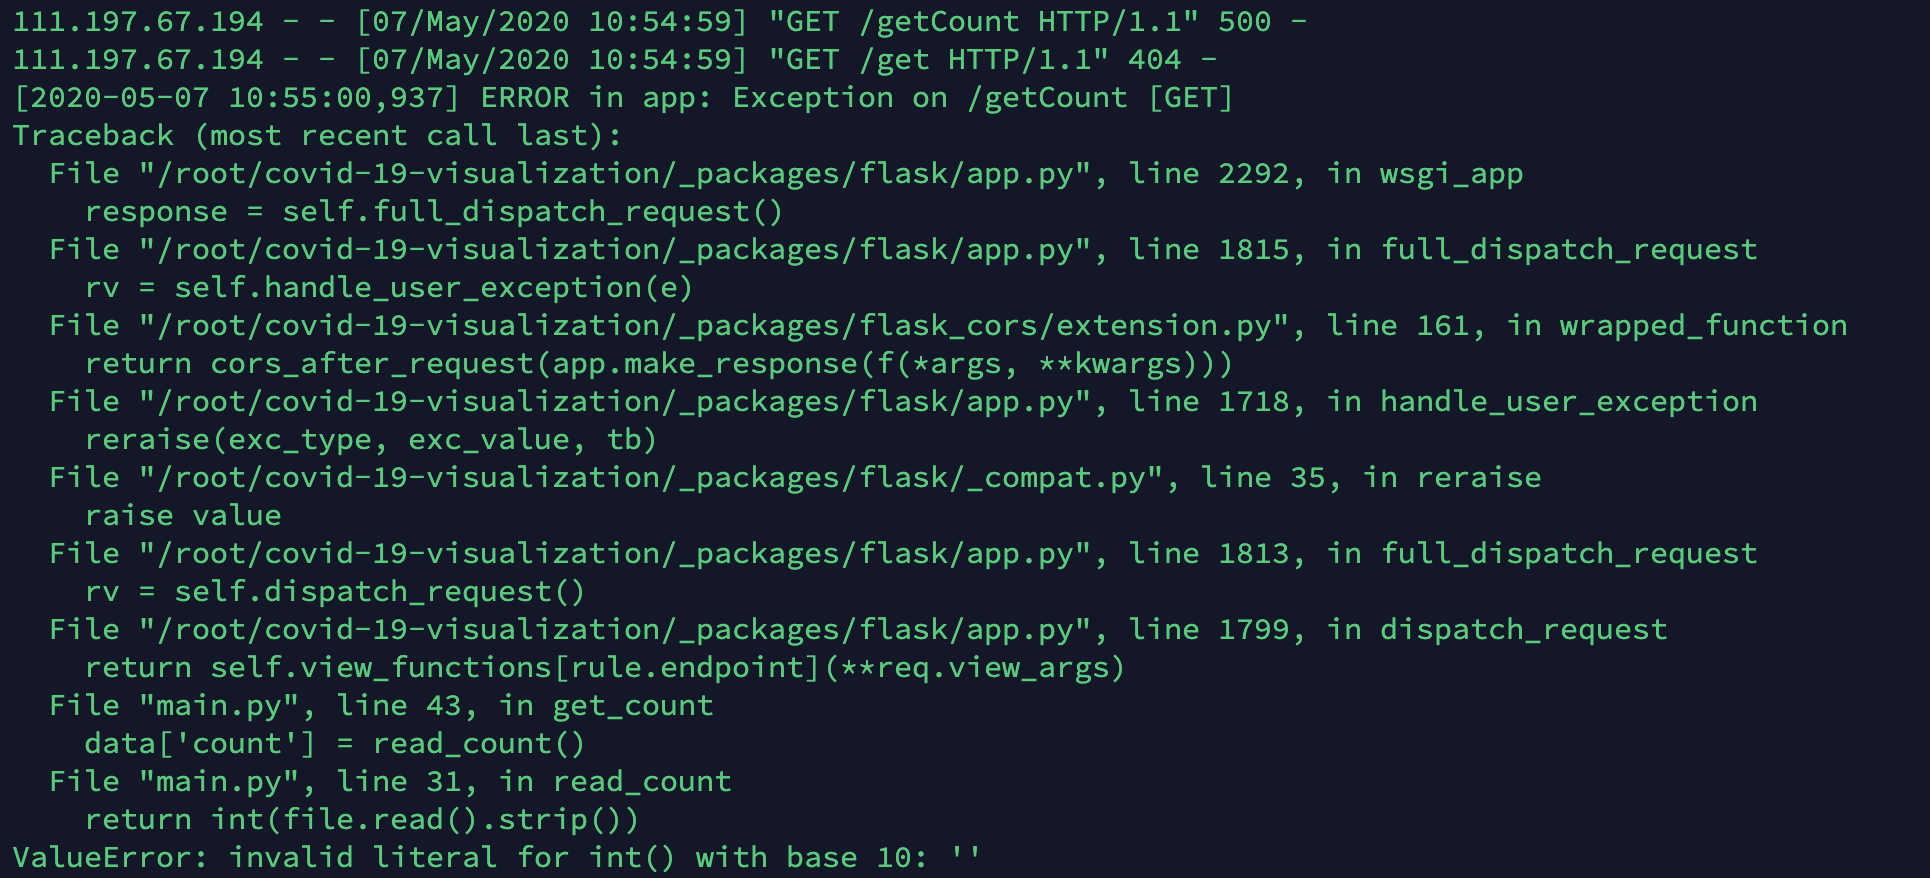
\includegraphics[width=0.8\textwidth]{pic3.png}
\end{figure}

出现该问题是因为某些记录文件被误删除而导致了无法读取数据。发现问题后,我们马上对代码进行修缮,解决了这个问题。

通过站点访问日志,我们可以从整体上了解后端的健康情况,及时发现站点中存在的一些“边界”问题。

\subsubsection{数据访问与更新日志}
后端的重点在于数据的维护,因此数据访问与更新的日志是十分重要的。我们在数据访问与更新日志中记录了每一次向后端申请数据的时间、内容和结果,同时也记录了每一次后端向网络请求数据更新的结果与得到更新数据后数据库更新的结果。下图为部分记录。

\begin{figure}[H]
\centering
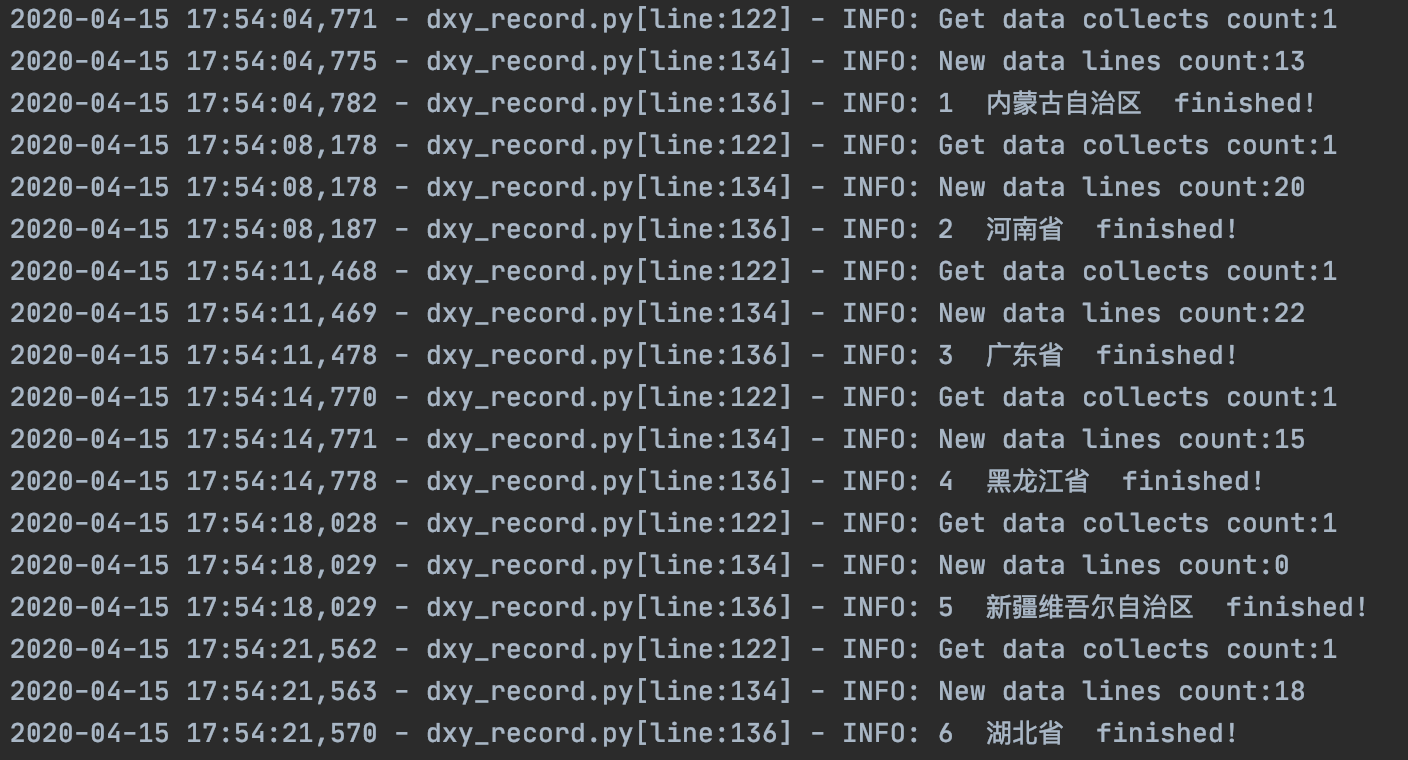
\includegraphics[width=0.8\textwidth]{pic4.png}
\end{figure}

为了更好的了解数据访问与更新情况,我们将日志设置了三个等级:“debug”、“information”和“wrong”。

Debug等级是我们在编写代码测试时使用的一种极其详细的日志等级,因为日志十分冗余,在项目上线运行时一般不需要查看该等级的日志。

Information等级是项目运行时记录访问与更新情况用的较多的一个等级,在该等级中,我们会详细记录每一次的后端操作的信息,例如上图就是数据更新操作的Information等级日志。

Wrong等级日志是项目运行时记录我们认为不应该出现的情况,例如“向网络请求数据更新得到空条目”,在中期报告不久后的时间,我们发现虽然后端数据自动更新的程序在运行着,但是数据库内数据停滞更新了,通过查看日志我们发现,时原来使用的某个API接口停止服务了,得到该信息后,我们迅速修改了更新的相关流程,将后端数据更新。


\subsubsection{日志的部署与记录方式}
项目后端的重点是数据的维护,面对庞大的维护信息,日志记录是一个强大的助手,因此我们十分重视日志记录,在项目开始时就部署了以上两部分日志。

为了方便及时阅读,后端的日志是以纯文本的方式记录的,不同方面,不同等级的日志分别处于不同的文件中,我会在本机运行Python程序定时将远程服务器的日志文件拷贝到本机进行异常检查,以便及时发现问题,修复问题。


\subsubsection{日志量}

站点访问日志根据我们站点的访问次数而定,每有一次访问时会增加一条记录,因此日志数量并不固定。

由于后端的数据自动更新程序每30分钟会网络请求数据更新,因此数据访问与更新日志中的Information等级日志日志量较大,达到约每天6000行左右,其中记录数据更新的日志占90\%左右。

数据访问与更新日志中的Wrong等级日志主要记录后端中的异常情况,现在我们的项目已经稳定的运行,因此日志量较小,近一周平均每天约7.3行。

数据访问与更新日志中的Debug等级日志主要为调试代码使用,因此不在此讨论日志量。

\subsection{前端的日志}
前端通过nginx实现持续挂载,在初步实现挂载时开始进行日志记录,对访问信息日志$access.log$和错误信息日志$error.log$进行维护,均保存在nginx服务器的日志保存目录中。
\subsubsection{访问日志}
访问日志主要包括如下具体内容:(1) 客户端(具体用户)IP地址,例如一开始主要是“222.185.220.44”,这是本组前端维护者的IP,之后地址逐渐多样化,代表开始在用户中得到推广;(2) 访问时间;(3) 请求的URL地址、请求状态、请求页面大小; (4) 请求页面大小; (5) 来源页面; (6)浏览器信息
我们目前通过简单的离线执行的(非实时运行)代码,从访问日志中作两类信息的利用:统计用户来源;数据传输量。数据传输量是为了下一步进行性能优化作参考。
下图为部分记录
\begin{figure}[H]
\centering
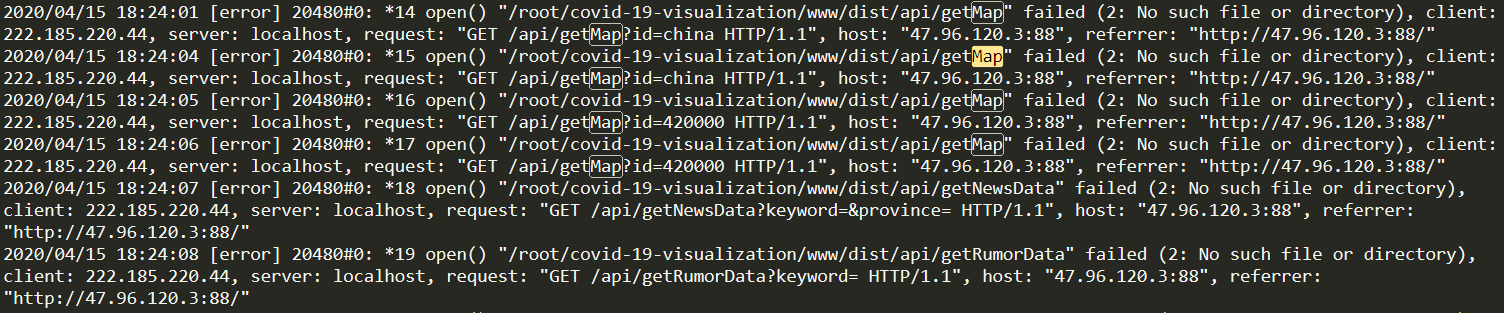
\includegraphics[width=0.8\textwidth]{access.png}
\end{figure}
\subsubsection{错误日志}
错误日志重点内容在于错误信息,主要结合其中的请求内容、错误提示观察其中的错误类型,目前遇到的问题主要为两类:重新build导致暂时的文件缺失、后端调整导致的访问失败。
下图为部分记录
\begin{figure}[H]
\centering
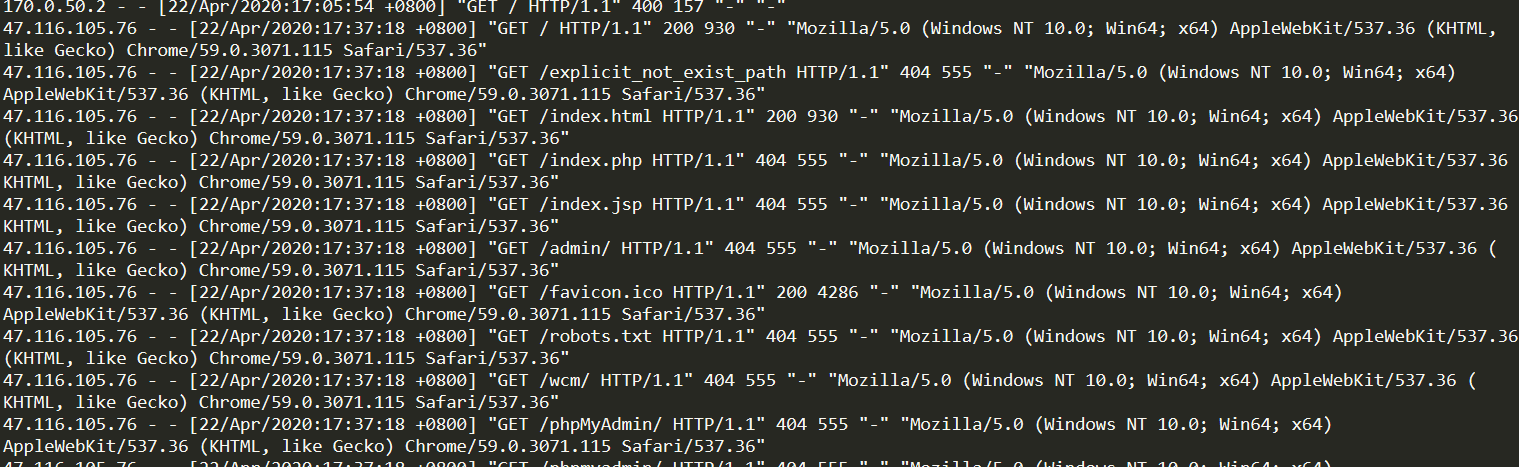
\includegraphics[width=0.8\textwidth]{error.png}
\end{figure}
\subsubsection{日志的部署与记录方式}
前端通过nginx实现持续挂载,在初步实现挂载时开始进行日志记录,对访问信息日志access.log和错误信息日志error.log进行维护,均保存在nginx服务器的日志保存目录中
\subsubsection{日志量}
目前错误日志大约共一百余条,均为调整产生;访问日志日均30条。我们近期参考已有的实现方式,进行日志切割,按日期进行存放。

\section{计数接口介绍}

在本项目中按要求增加了一个计数器接口:

$$http://47.96.120.3:9400/getCount$$

该计数器主要计量后端接口的调用次数,例如“用户查看了北京地区的疫情数据”,“用户使用关键词搜索了一次新闻”和“用户判断了一次谣言”等。

当访问该接口时,会按要求返回按照$\{"count": 42\}$格式的数据。

\section{进展总结}

\subsection{遇到的问题}
我们发现了一些前端的界面设计原则、优秀的前端设计产品,目前需要结合我们的Feature进行设计。
下一阶段是我们组可选任务的实现阶段,我们最初制订了两条可选任务:“关联推荐:推荐官方已辟谣、证实的消息”、“结合关键词判断谣言”,目前第一条已经完成,第二条正在实现。但我们发现我们产品目前还需要对舆论输入的有更好的利用,最初制定的可选任务需要调整。
\subsection{未来计划}
对下两周可选任务进行调整,计划上线舆论热度可视化功能,完善产品。
后端部分未来着手负载相关的问题,提高网站的鲁棒性。
\end{document}